\documentclass{ctexart}
\usepackage{graphicx}
\usepackage{amsmath}
\usepackage{amssymb}
\usepackage{hyperref}
\usepackage{geometry}
\usepackage{enumitem}
\usepackage{booktabs}
\usepackage{xcolor}
\usepackage{placeins}
\usepackage{float}
\hypersetup{hidelinks}
\geometry{a4paper, left=1in, right=1in, top=1in, bottom=1in}

\newcommand{\missingresult}{--}

\title{《深度学习基础》第四次实验报告}
\author{PB24000150 李欣宸}
\date{\today}

\begin{document}

\maketitle

本文是《深度学习基础》的第四次实验报告。代码实现在 \verb|lab/lab4| 目录下，实验目标是使用 SimCLR 框架在 CIFAKE 数据集上进行真实图像与 AI 生成图像检测。报告内容包含 SimCLR 预训练、冻结线性评估，并选择 3 个附加实验：不同对比学习损失、Projection Head 结构分析和超参数分析。

本实验主要使用学校本科生算力平台服务器中的 RTX 5090 GPU 进行训练，最终实验结果均记录在 Swanlab 上。

\section{实验设计}

\subsection{实验设置}

\paragraph{数据集}
本实验使用 CIFAKE 数据集。该数据集包含 CIFAR-10 真实图像和 Stable Diffusion 生成图像，任务为二分类：真实图像与 AI 生成图像。原始图像大小为 $32\times 32$，输入为 RGB 三通道。

本实验中只使用了测试集和训练集，不使用验证集，因为该任务主要衡量预训练习得表征的质量，分类器是简单的线性分类器，所以在统一数据分割比例下，训练准确率的相对大小能有效地衡量预训练的效果。

\begin{table}[htbp]
    \centering
    \begin{tabular}{lccc}
        \toprule
        设置 & 无监督预训练样本数 & 冻结评估带标签样本数 & 测试样本数 \\
        \midrule
        1\% 标签（\verb|r1|） & 49500 & 500 & 10000 \\
        10\% 标签（\verb|r10|） & 45000 & 5000 & 10000 \\
        \bottomrule
    \end{tabular}
    \caption{数据划分}
    \label{tab:data-split}
\end{table}

\paragraph{数据增强}
SimCLR 的核心是把同一张图像的两次随机增强结果作为正样本对。本实验使用的增强包括随机裁剪、水平翻转、颜色扰动、随机灰度化和可选的高斯模糊。随后使用 CIFAR-10 的均值和方差进行标准化。图 \ref{fig:augmentation-effects} 展示了不同增强方式对样本的影响。

\begin{figure}[H]
    \centering
    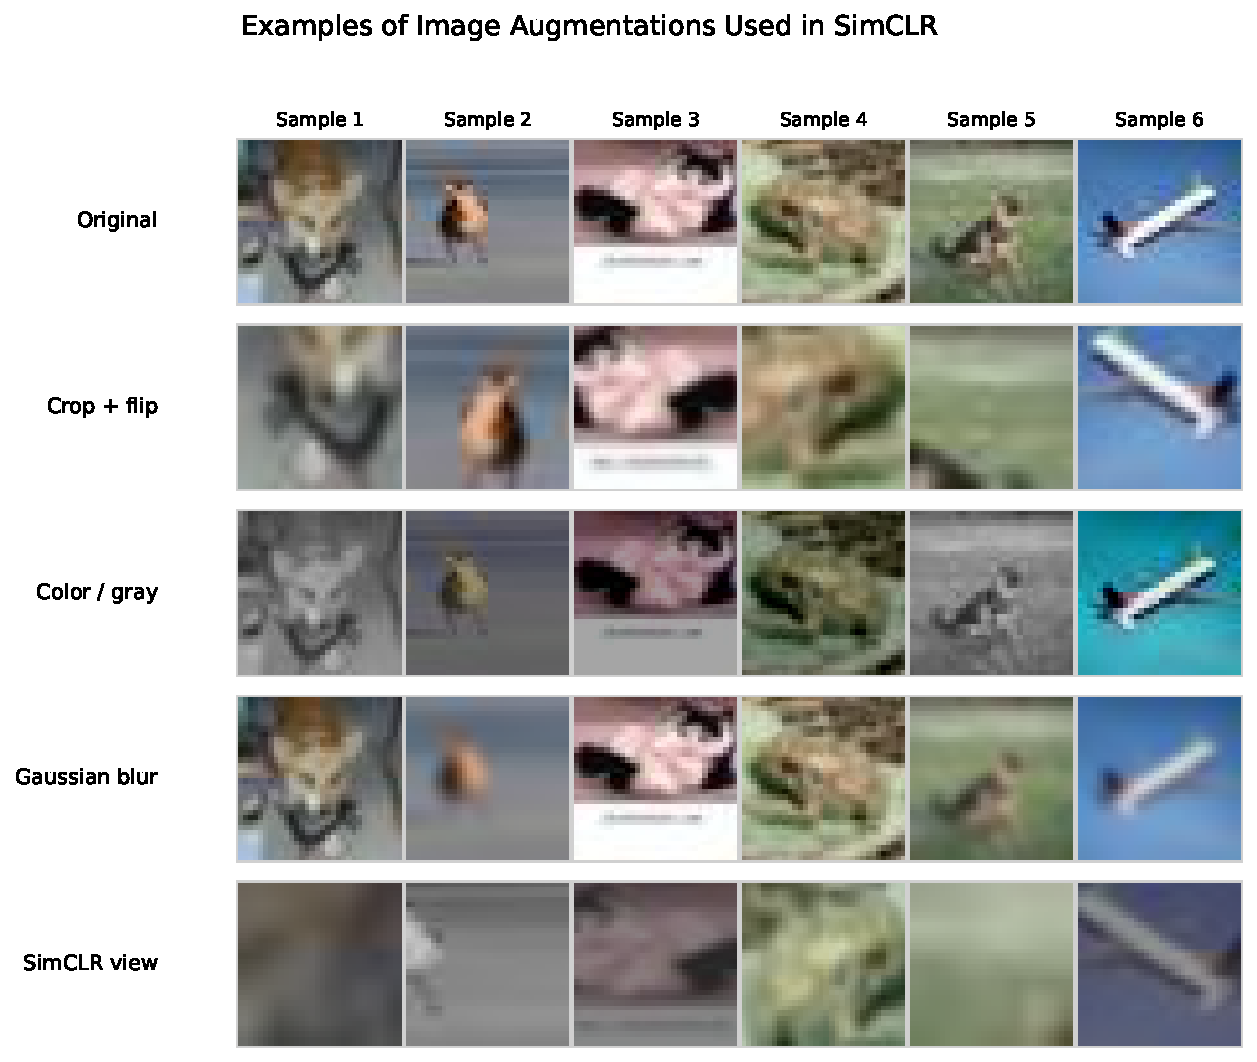
\includegraphics[width=0.95\linewidth]{figures/augmentation_effects.pdf}
    \caption{数据增强效果示例}
    \label{fig:augmentation-effects}
\end{figure}

\paragraph{训练设置}
无监督预训练阶段使用 AdamW 优化器，默认学习率为 $10^{-3}$，温度系数 $\tau=0.5$，Projection Head 输出维度为 64。主实验比较 ResNet-18 和 MobileNetV2 两种 encoder；ResNet-18 的 \verb|r1| 设置训练 1000 个 epoch，其余主实验设置训练 500 个 epoch，默认预训练 batch size 为 2048。冻结评估阶段固定 encoder 参数，只提取 encoder 特征，并在这些特征上，使用 Logistic 回归训练一个单层线性分类器。

Baseline 则不进行 SimCLR 预训练，直接从随机初始化的 encoder 开始，用 1\% 或 10\% 的带标签数据端到端训练二分类模型。

\subsection{模型架构}

\paragraph{Encoder}
实验模型的 Encoder 基于 ResNet-18 和 MobileNetV2 两种经典卷积神经网络架构。为了适配 CIFAKE 的 $32\times32$ 输入图像，两种模型经过了以下修改：

\begin{itemize}[noitemsep]
    \item ResNet-18：将第一层卷积改为 $3\times3$、stride 为 1，并去掉原始的 max pooling，以适配 $32\times32$ 的 CIFAKE 图像；最终去掉分类层，输出 512 维特征。
    \item MobileNetV2：将第一层卷积 stride 改为 1，并去掉原始分类器；最终输出 1280 维特征。
\end{itemize}

这两个 encoder 的设计目标不同。ResNet-18 通过残差连接提升深层网络的可训练性；MobileNetV2 使用倒残差结构和深度可分离卷积，在参数量和计算量上更轻量。主实验中同时记录两种 encoder 的 SimCLR 预训练与冻结评估结果。

\paragraph{Projection Head}
SimCLR 不直接在 encoder 特征上计算对比损失，而是先将特征输入 Projection Head。实验中 Projection Head 为两层 MLP：
\[
    h = f_\theta(x), \quad
    z = g_\phi(h) = W_2 \sigma(\operatorname{BN}(W_1h)).
\]
其中 $h$ 是 encoder 输出的表征，$z$ 是用于计算对比损失的投影向量。默认隐藏层维度为 128，输出维度为 64，并启用 BatchNorm。冻结评估时丢弃 Projection Head，只使用 encoder 输出 $h$。

\subsection{实验原理}

\subsubsection{SimCLR}

SimCLR \cite{chen2020simclr} 是一种简单的对比学习框架。对 batch 中每张图像 $x_k$，随机增强两次得到 $x_{2k-1}$ 和 $x_{2k}$，这两个 view 构成正样本对；同一 batch 中其他图像的 view 构成负样本。模型通过 encoder $f_\theta$ 和 projection head $g_\phi$ 得到投影向量：
\[
    z_i = g_\phi(f_\theta(x_i)).
\]

训练目标是让同一图像的两个增强 view 在表示空间中靠近，让不同图像的 view 远离。由于没有使用标签，预训练阶段能利用大量无标签图像学习通用视觉表示。

\subsubsection{NT-Xent 损失}

本实验手动实现了 SimCLR 中常用的 NT-Xent 损失。设 batch 中原始样本数为 $N$，增强后共有 $2N$ 个 view。对正样本对 $(i,j)$，其单向损失为
\[
    \ell_{i,j}
    =
    -\log
    \frac{\exp(\operatorname{sim}(z_i,z_j)/\tau)}
    {\sum_{k=1}^{2N}\mathbb{1}_{k\ne i}\exp(\operatorname{sim}(z_i,z_k)/\tau)},
\]
其中 $\operatorname{sim}$ 为余弦相似度，$\tau$ 为温度系数。最终 loss 为所有正样本对两个方向损失的平均：
\[
    \mathcal{L}
    =
    \frac{1}{2N}
    \sum_{k=1}^{N}
    \left(
    \ell_{2k-1,2k} + \ell_{2k,2k-1}
    \right).
\]

在实现中，先将 $z_1,z_2$ 拼接为 $2N$ 个向量，并进行 $L_2$ 归一化；再计算完整相似度矩阵，将对角线置为 $-\infty$ 排除自身匹配；标签通过偏移 $N$ 的方式构造，使每个 view 的正样本都是同一图像的另一个 view。

\subsubsection{冻结评估与 Baseline}

预训练完成后，我们使用 1\% 和 10\% 标签数据，拟合一个简单的 Logistic 回归分类器，再在训练集和测试集上评估 Accuracy 和 F1。

Baseline 则直接从随机初始化的 encoder 开始，使用相同的带标签数据端到端训练分类器。对比 SimCLR 预训练的结果与 baseline，可以评估预训练是否从无标签的训练中学到了有用的表示，使得习得的特征具有较好的线性可分性。

\section{结果与讨论}

\subsection{主实验结果}

主实验的已完成结果见表 \ref{tab:main-results}。图 \ref{fig:main-pretrain-curves} 展示了 ResNet-18 和 MobileNetV2 在 \verb|r1| 与 \verb|r10| 两个设置下的 SimCLR 预训练曲线。\footnote{由于 end2end 和 SimCLR 的训练方式不同，其 epoch 数不可直接比较，Baseline 的准确率有明显的震荡和过拟合现象，因此只取 100 epoch。}

\begin{table}[H]
    \centering
    \begin{tabular}{llcccc}
        \toprule
        Encoder & 方法 & 标签比例 & Test Acc & Test F1 & 备注 \\
        \midrule
        ResNet-18 & Baseline & 1\% & 0.8046 & 0.8086 & 100 epoch \\
        ResNet-18 & SimCLR + linear probe & 1\% & 0.9576 & 0.9580 & 1000 epoch \\
        ResNet-18 & Baseline & 10\% & 0.9038 & 0.9075 & 100 epoch \\
        ResNet-18 & SimCLR + linear probe & 10\% & 0.9603 & 0.9604 & 500 epoch \\
        MobileNetV2 & SimCLR + linear probe & 1\% & 0.9159 & 0.9166 & 500 epoch \\
        MobileNetV2 & SimCLR + linear probe & 10\% & 0.9232 & 0.9233 & 500 epoch \\
        \bottomrule
    \end{tabular}
    \caption{不同 encoder 与标签比例下的主实验结果}
    \label{tab:main-results}
\end{table}

\begin{figure}[H]
    \centering
    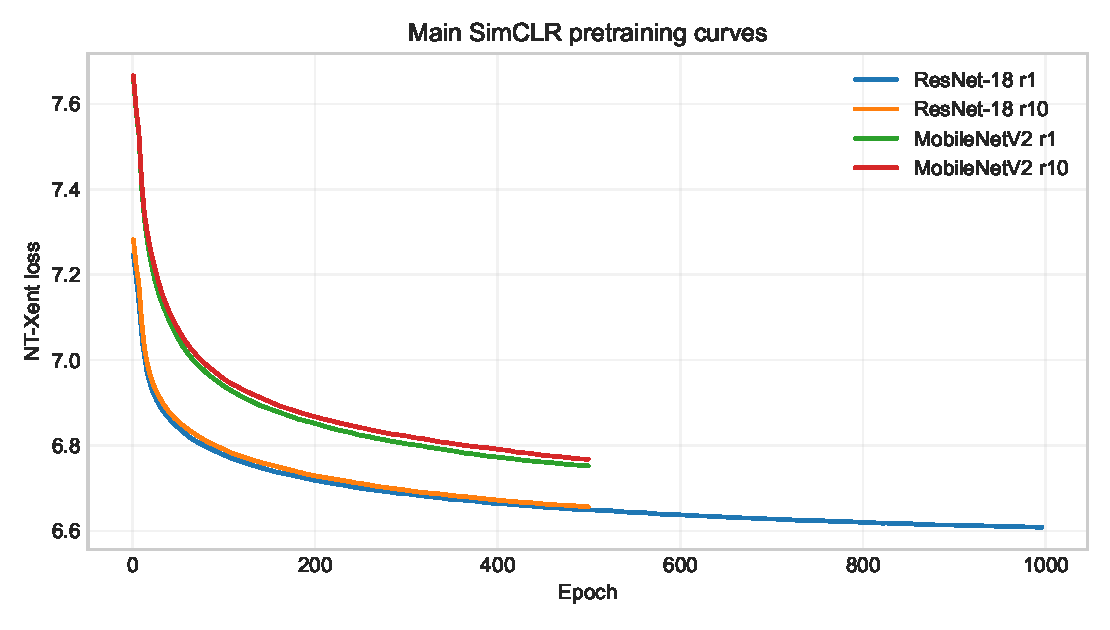
\includegraphics[width=0.95\linewidth]{figures/main_pretrain_curves.pdf}
    \caption{主实验 SimCLR 预训练曲线}
    \label{fig:main-pretrain-curves}
\end{figure}
\FloatBarrier

从结果看，ResNet-18 在 1\% 和 10\% 标签下的冻结评估结果都接近 0.96，说明 SimCLR 预训练后的表示在真实/生成二分类上已经比较线性可分。MobileNetV2 的结果低于 ResNet-18，1\% 和 10\% 标签下的 F1 分别为 0.9166 和 0.9233，但仍显著高于 1\% 标签下从头训练的 ResNet-18 baseline。这说明在当前实现中，ResNet-18 对 CIFAKE 的真实/生成线索捕捉更有效；MobileNetV2 虽然更轻量，但其深度可分离卷积和更强的结构约束可能限制了对细粒度纹理、颜色统计等线索的表达。

从曲线看，预训练 loss 一直稳定地下降，即使到 1000 个 epoch，训练仍然没有收敛，暗示当训练轮数增加，效果会越来越好，训练瓶颈主要在于时间和算力。

\subsection{附加实验一：不同对比学习损失}

除 NT-Xent 外，代码还实现了 logistic-style contrastive loss 和 Triplet Loss。三种损失的区别如下：

\begin{itemize}[noitemsep]
    \item NT-Xent：使用 batch 内全部其他 view 作为负样本，负样本数量随 batch size 增大而增加，是 SimCLR 的标准选择。
    \item Logistic contrastive loss：将 view 两两相似度视为二分类 logits，正样本位置目标为 1，其余位置为 0，优化方式更直接，但对负样本间的相对排序约束较弱。
    \item Triplet Loss：每个 anchor 只使用一个正样本和一个负样本，目标是让正样本距离至少比负样本距离小一个 margin；实现简单，但负样本利用效率低。
\end{itemize}

结果见表 \ref{tab:loss-results} 和图 \ref{fig:loss-pretrain-curves}。三种 loss 的数值尺度不同，预训练 loss 不能横向直接比较；图中把每条曲线按该实验的初始值和最终值归一化，只用于比较下降趋势。更有意义的结果仍然是冻结评估后的 Accuracy 和 F1。

\begin{table}[H]
    \centering
    \begin{tabular}{lcccc}
        \toprule
        Loss & 最终预训练 loss & Test Acc & Test F1 & 备注 \\
        \midrule
        NT-Xent & 6.6552 & 0.9603 & 0.9604 & 标准 SimCLR \\
        Logistic & 0.7001 & 0.6376 & 0.6425 & 相似度矩阵二分类 \\
        Triplet & 0.1484 & 0.9471 & 0.9475 & 单负样本 margin \\
        \bottomrule
    \end{tabular}
    \caption{不同对比学习损失的结果}
    \label{tab:loss-results}
\end{table}

\begin{figure}[H]
    \centering
    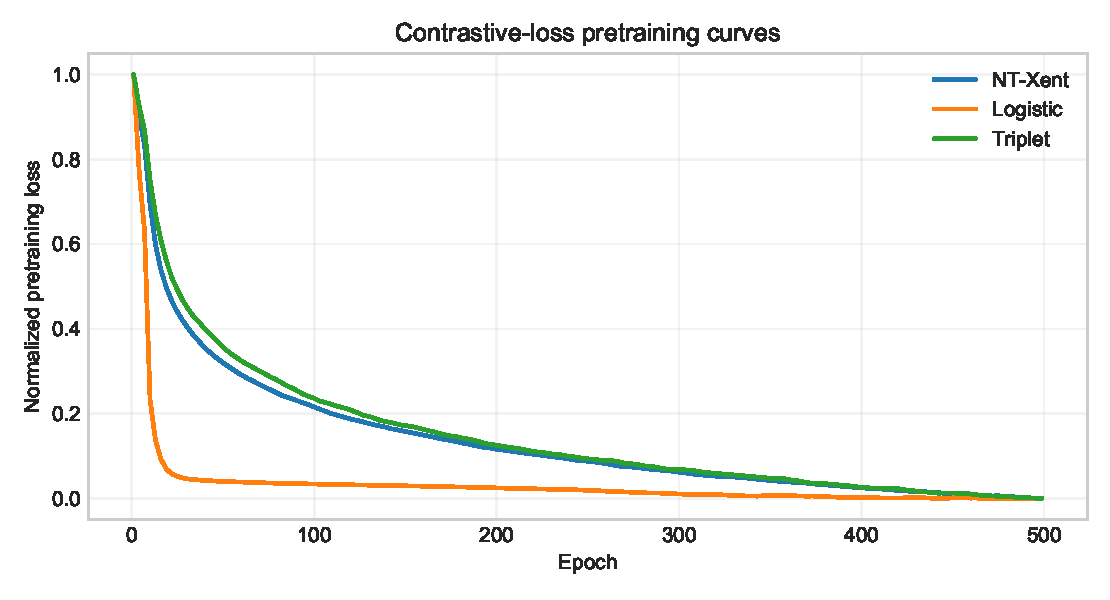
\includegraphics[width=0.95\linewidth]{figures/loss_pretrain_curves.pdf}
    \caption{不同对比学习损失的归一化预训练曲线}
    \label{fig:loss-pretrain-curves}
\end{figure}

NT-Xent 的结果最好，Triplet Loss 略低但仍然可用，而 Logistic contrastive loss 明显失败。这是因为 Triplet Loss 每次只显式使用一个负样本，负样本利用效率较低，训练速度更慢；但是从训练趋势看，如果延长训练时间，Triplet Loss 的训练有希望达到更好的效果。而 Logistic contrastive loss 的失败可能在于 margin 设置的不合理，以及对 batch 中负样本的利用率过低，具体原因由于实验时间原因我没有深入分析。
\FloatBarrier

\subsection{附加实验二：Projection Head 结构分析}

Projection Head 的作用不是直接提高分类器容量，而是让 encoder 的表示 $h$ 和对比损失使用的表示 $z$ 分开。这样可以把对比学习中由数据增强带来的不变性更多地压到 $z$ 空间中，而保留 $h$ 中对下游任务有用的信息。

本实验比较 BatchNorm、隐藏层维度和输出维度对冻结评估的影响，结果见表 \ref{tab:head-results}。所有设置都使用 ResNet-18、\verb|r10|、$\tau=0.5$ 和 batch size 2048。

\begin{table}[H]
    \centering
    \begin{tabular}{lcccc}
        \toprule
        Projection Head & Hidden dim & Projection dim & Test Acc & Test F1 \\
        \midrule
        Linear-ReLU-Linear & 128 & 64 & 0.9548 & 0.9549 \\
        Linear-BN-ReLU-Linear & 128 & 64 & 0.9603 & 0.9604 \\
        Linear-BN-ReLU-Linear & 256 & 64 & 0.9560 & 0.9562 \\
        Linear-BN-ReLU-Linear & 128 & 128 & 0.9575 & 0.9576 \\
        \bottomrule
    \end{tabular}
    \caption{Projection Head 结构对冻结评估结果的影响}
    \label{tab:head-results}
\end{table}

从结果看，加入 BatchNorm 的默认结构最好，不加 BatchNorm 的 F1 下降到 0.9549，说明投影空间的尺度稳定性确实会影响对比学习效果。隐藏层从 128 增大到 256 没有带来提升，projection dim 从 64 增大到 128 也略有下降。这说明在本任务中，head 容量不是越大越好；过强的 projection head 可能更多地吸收对比学习目标，使 encoder 本身的线性可分性提升有限。

\subsection{附加实验三：超参数分析}

SimCLR 对 batch size 和温度系数比较敏感。Batch size 越大，每个 anchor 能看到的负样本越多，通常有利于对比学习；温度系数控制相似度分布的尖锐程度，$\tau$ 较小时模型更强调 hardest negatives，但训练也可能更不稳定。

本实验比较不同温度系数与 batch size，结果见表 \ref{tab:hyper-results} 和图 \ref{fig:hyper-pretrain-curves}。

\begin{table}[H]
    \centering
    \begin{tabular}{lcccc}
        \toprule
        设置 & Temperature & Batch size & Test Acc & Test F1 \\
        \midrule
        默认 & 0.5 & 2048 & 0.9603 & 0.9604 \\
        低温度 & 0.1 & 2048 & 0.9445 & 0.9449 \\
        较高温度 & 1.0 & 2048 & 0.9612 & 0.9613 \\
        小 batch & 0.5 & 512 & 0.9626 & 0.9627 \\
        更小 batch & 0.5 & 256 & 0.9654 & 0.9657 \\
        \bottomrule
    \end{tabular}
    \caption{温度系数和 batch size 对结果的影响}
    \label{tab:hyper-results}
\end{table}

\begin{figure}[H]
    \centering
    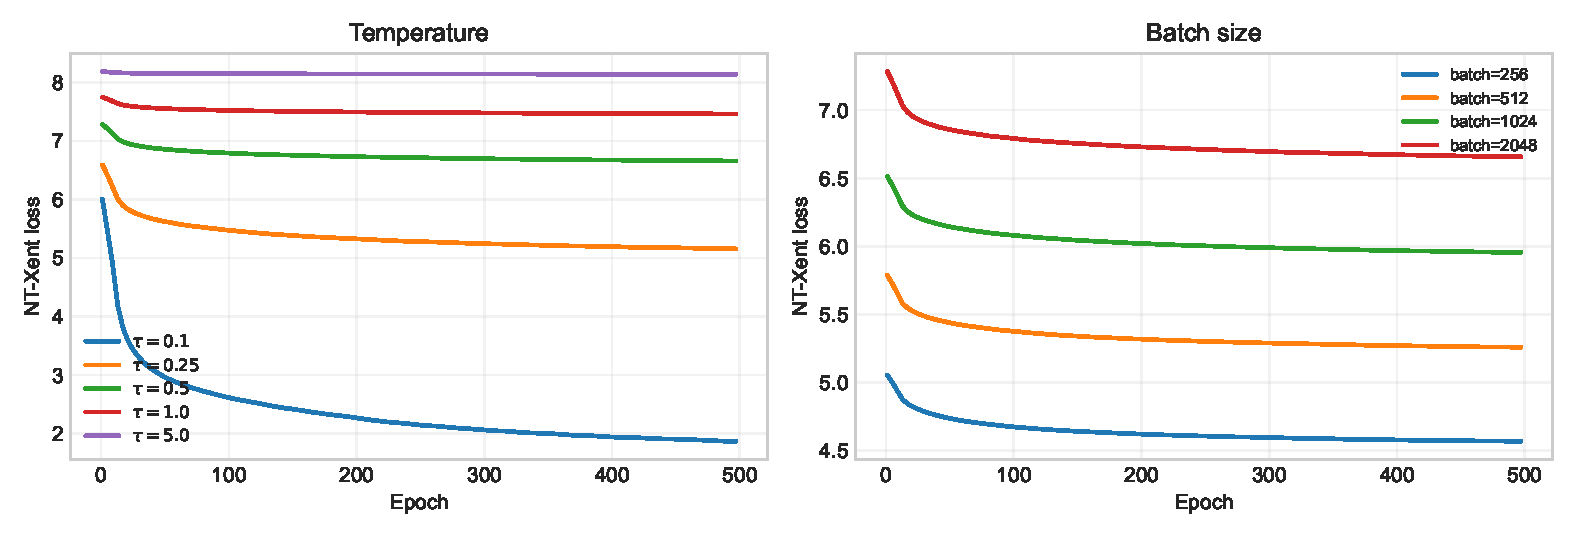
\includegraphics[width=0.95\linewidth]{figures/hyper_pretrain_curves.pdf}
    \caption{温度系数和 batch size 对预训练曲线的影响}
    \label{fig:hyper-pretrain-curves}
\end{figure}

温度系数的影响比较明显。$\tau=0.1$ 时结果下降到 0.9449 F1，说明过低温度会让 softmax 过度关注少数困难负样本，训练目标变得尖锐；$\tau=1.0$ 与默认 $\tau=0.5$ 接近，略好于默认设置；继续增大到 2.5 或 5.0 的实验也运行过，但 F1 分别只有约 0.9492 和 0.9462，因此没有列入表中。

Batch size 的结果与 SimCLR 原论文中的结论有所出入：batch size 从 2048 降到 512、256 后，冻结评估反而略有提升。这可能与 CIFAKE 的任务特点有关。真实/生成图像的差异主要并不在于语义差异，过大的 batch 提供更多负样本，但也会更强地推动不同图像在表示空间中分散，未必总能保留对 AIGC 检测有用的纹理和统计线索。

另外可以观察到，$\log (\text{Batch size})$ 和 Loss 的大小之间存在线性关系，这是因为：

\begin{equation}
    \ell_{i,j}
    =
    -\log
    \frac{\exp(\operatorname{sim}(z_i,z_j)/\tau)}
    {\sum_{k=1}^{2N}\mathbb{1}_{k\ne i}\exp(\operatorname{sim}(z_i,z_k)/\tau)}
    \approx
    -\log
    \frac{1}
    {2N-1}
    =
    \log(2N-1).
\end{equation}

而 Temperature 的影响则呈现出明显的非线性，这可能与任务特性和数据增强策略有关。

\subsection{讨论}

CIFAKE 检测与普通 CIFAR-10 分类不同，类别标签不是物体语义，而是真实图像和生成图像的来源差异。因此，模型可能依赖颜色统计、局部纹理、频域伪影等线索。SimCLR 的数据增强会主动抹去部分颜色和纹理信息，这对一般语义表征是有益的，但对 AIGC 检测未必总是有益。尤其是随机裁剪过强时，$32\times32$ 小图像中的局部统计容易被破坏；颜色扰动过强时，生成图像的颜色分布差异也可能被削弱。

因此，本实验的结果意义可能较为有限。NT-Xent 和 Triplet Loss 的差异并不明显，略好于 baseline 的结果也不能完全说明 对比学习的优势，但是这作为一次为了帮助同学们了解 SimCLR 框架而设计的实验还是相对成功的。

\section{结论}

本实验实现了基于 SimCLR 的 AIGC 生成图像检测流程，包括双视角数据增强、ResNet-18 和 MobileNetV2 encoder、Projection Head、NT-Xent 损失、冻结线性评估和从头训练 baseline。已完成的 ResNet-18 SimCLR 实验在 1\% 和 10\% 标签下都取得了约 0.96 的 Test F1，说明自监督预训练学到的表示对 CIFAKE 二分类有效。

附加实验中，NT-Xent 明显优于 Logistic contrastive loss，也略优于 Triplet Loss；默认带 BatchNorm 的两层 projection head 效果最好；温度系数过低会损害结果，而较小 batch size 在本任务中反而略好。

\begin{thebibliography}{9}

\bibitem{chen2020simclr}
Chen, T., Kornblith, S., Norouzi, M., and Hinton, G. A Simple Framework for Contrastive Learning of Visual Representations. ICML, 2020.

\bibitem{he2016resnet}
He, K., Zhang, X., Ren, S., and Sun, J. Deep Residual Learning for Image Recognition. CVPR, 2016.

\bibitem{sandler2018mobilenetv2}
Sandler, M., Howard, A., Zhu, M., Zhmoginov, A., and Chen, L.-C. MobileNetV2: Inverted Residuals and Linear Bottlenecks. CVPR, 2018.

\end{thebibliography}

\end{document}
